\documentclass[hyperref={pdfpagelabels=false}]{beamer}
%%% workaround: http://tex.stackexchange.com/questions/4436/beamer-undefined-control-sequence
\providecommand\thispdfpagelabel[1]{}
%%%
\usepackage{beamerthemesplit}
\usepackage{lmodern}
\title{Using linux at UIC}
\author{UIC Linux Users Group}
\date{\today}
\begin{document}
\frame{\titlepage}
\section{Wireless}
\subsection{About WPA2-Enterprise}
\frame
{
    \frametitle{Wi-Fi Protected Access II Enterprise}
    \begin{itemize}
    \item{WPA2 is the finalized version of the IEEE 802.11i standard, added AES-CCMP encryption, and has been in place since 2004}
    \item{Per user Authentication}
    \item{Also referred WPA-802.1X mode}
    \end{itemize}
}
\subsection{Network Manager}
\frame
{
    \frametitle{Network Manager}
    
    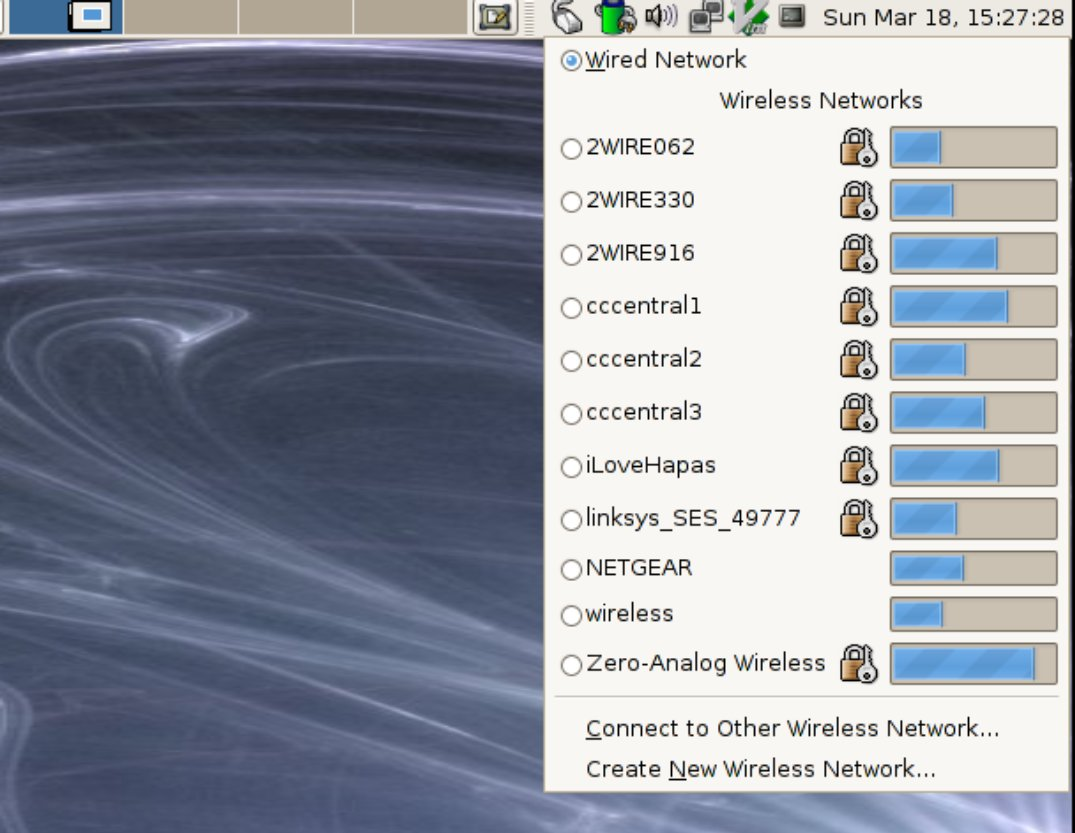
\includegraphics[totalheight=0.7\textheight]{gnm.jpg}

}
\frame
{
    \frametitle{connecting to the network}
    http://acm.cs.uic.edu/uicwifi-linux

    security: WPA and  WPA2 Enterprise
}
\subsection{Wireless Settings}
\frame
{
     \frametitle{network settings} 
     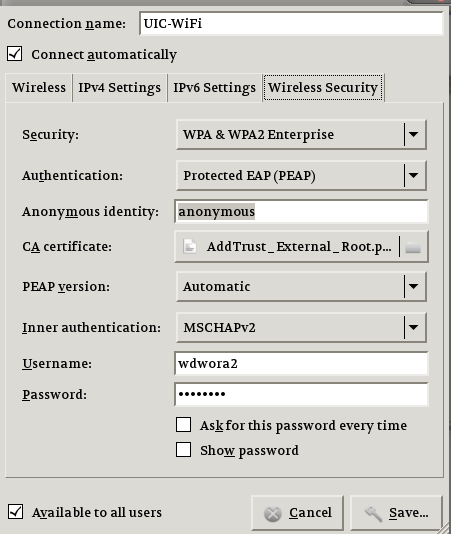
\includegraphics[totalheight=0.8\textheight]{uicwificonfig.png}
}
\frame
{
    \frametitle{network settings}
    \begin{itemize}
    \item{Network name: UIC-WiFi}
    \item{Wireless Security: WPA \& WPA2 Enterprise}
    \item{Authentication: PEAP}
    \item{Anonymous Identity: anonymous}
    \item{CA Cert: AddTrust\_External\_Root}
    \item{inner Authentication: MSCHAPv2}
    \item{Username: ACCC NETID}
    \item{Password: ACCC PASSWORD}
    \end{itemize}
}
\frame
{
    \frametitle{Pray}
    Pray...
}
\section{Printing}
\subsection{Pharos}
\frame
{
    \frametitle{Pharos}
    Pharos is ACCC's print management system at UIC.
}
\subsection{Setup}
\frame
{
    \frametitle{Setup}
     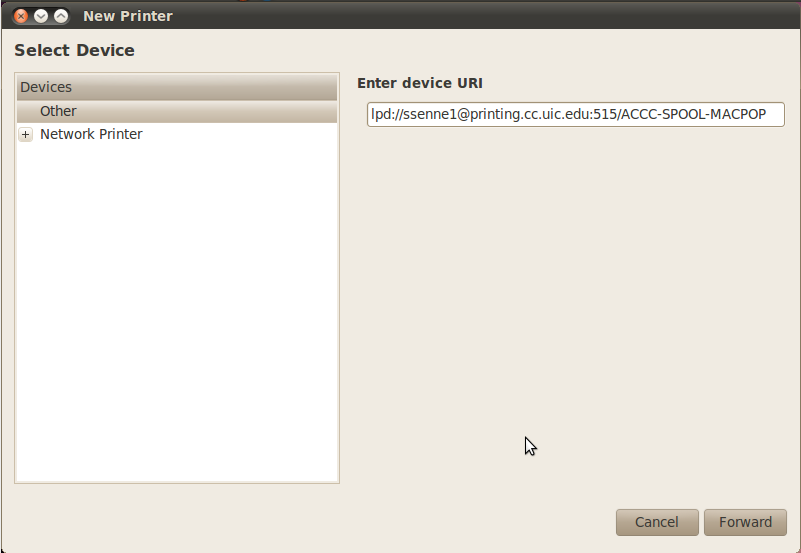
\includegraphics[totalheight=0.8\textheight]{PrinterURI.png}
}
\subsection{Select Printer Driver}
\frame
{
    \frametitle{Select Printer Driver}
     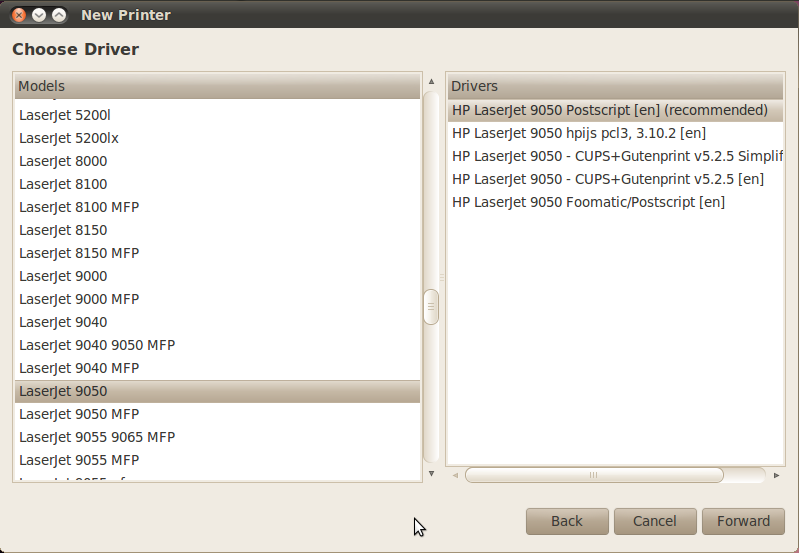
\includegraphics[totalheight=0.8\textheight]{PrinterDriver.png}
}
\frame
{
    \frametitle{Name Printer}
     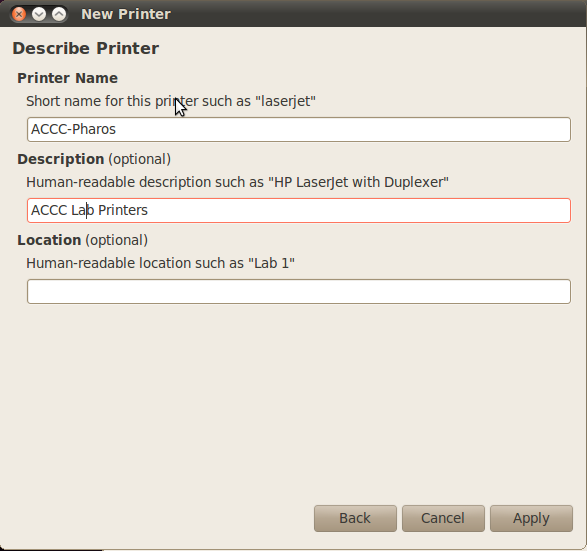
\includegraphics[totalheight=0.8\textheight]{PrinterName.png}

}
\subsection{Campus Housing}
\frame
{
	\frametitle{Campus Housing}
	To set up for UIC Housing printers, repeat this process for a new printer except the URI is "lpd://YOUR-NETID@printing.cc.uic.edu/ACCC-Spool-HousingPOP", the printer's make is "Lexmark", and the printer model is "Lexmark T645". If it is still not working, try going through the guide again and see if you missed something. If you still are having trouble, you can try dropping by the ACM to see if someone there can figure out what's wrong. 
}
\subsection{Summary}
\frame
{
    \frametitle{Summary}
URI: lpd://NETID@printing.cc.uic.edu:515/ACCC-SPOOL-MACPOP\\
Select printer from database: HP LaserJet 9050 Postscript en
Select Duplex if you want


}
\section{UIC Servers}
\frame
{
    \frametitle{UIC Servers}
    2 campus departments manage servers we have access to: ACCC and the CS department.
}
\subsection{Icarus}
\frame
{
    \frametitle{icarus.uic.edu}
    \begin{itemize}
    \item{ACCC server}
    \item{Status: RETIRED}
    \item{web hosting}
    \item{php, perl, bluestem, html}
    \item{shell access}
    \item{http://www2.uic.edu/$\sim$netid/}
    \item{Solaris}
    \end{itemize}
}
\subsection{Bert}
\frame
{
    \frametitle{Bert}
    \begin{itemize}
    \item{CS Department Server}
    \item{html}
    \item{Web hosting}
    \item{shell access}
    \item{http://cs.uic.edu/$\sim$cslogin/}
    \item{RHEL 5.9}
    \end{itemize}
}
\subsection{Ernie}
\frame
{
    \frametitle{Ernie}
    \begin{itemize}
    \item{CS Department Server}
    \item{html}
    \item{Web hosting}
    \item{shell access}
    \item{http://cs.uic.edu/$\sim$cslogin/}
    \item{RHEL 5.9}
    \end{itemize}
}
\subsection{People}
\frame
{
    \frametitle{People}
    \begin{itemize}
    \item{ACCC Hosting Service}
    \item{Must activate account: http://people.uic.edu/}
    \item{Web hosting}
    \item{SQLite (MySQL through another ACCC service)}
    \item{PHP, CGI, Ruby on Rails, Node.js, Python, etc}
    \item{shell access}
    \item{SMB network share}
    \item{http://$\sim$netid.people.uic.edu/}
    \item{RHEL 6.4 VM}
    \end{itemize}
}
\subsection{Webspace}
\frame
{
    \frametitle{How to use webspace}
    \begin{itemize}
    \item{create a $\sim$/public\_html directory}
    \end{itemize}
}
\section{Getting Help}

\subsection{ACCC}
\frame
{
	\frametitle{ACCC}
	The ACCC officially does not support linux, and will usually turn you away if
	seek assistance from them.
}
\frame
{
    \frametitle{Issues with ACCC}
    \begin{itemize}
    \item{ACCC account trouble}
    \item{windows/mac labs}
    \item{uic email}
    \item{wireless/resnet}
    \end{itemize}
}
\subsection{Contacting ACCC}
\frame
{
    \frametitle{Contacting ACCC}
    \begin{itemize}
    \item{talk to any ACCC consultant or lab monitor}
    \item{consult@uic.edu}
    \item{SEL 2267}
    \item{312-413-0003}
    \end{itemize}
}
\subsection{CS Department}
\frame
{
    \frametitle{Issues with CS department Computers}
    \begin{itemize}
    \item{If you don't know your account info}
    \item{If you your account info doesn't work}
    \item{If you need help using software}
    \item{If you need software installed for a class.}
    \end{itemize}
}
\subsection{Contacting CS Department}
\frame
{
    \frametitle{Contacting CS department}
    \begin{itemize}
    \item{pester Walter Dworak}

    
\includegraphics[totalheight=0.3\textheight]{wdwora2.jpg}
    \item{email support@cs.uic.edu}
    \end{itemize}
}
\end{document}
v
